\begin{frame}[standout]
    Extra slides
\end{frame}



\begin{frame}{Reference cell (buffer gas \& cell size)}

    Collision with untreated walls of the reference cell can depolarize the spin of electrons, forcing them to return to the ground state.

    To avoid this, we can either \textbf{add a buffer gas to reduce the number of collisions} composed of a mixture of $N_2$, $Ne$, $Ar$, and $He$ or \textbf{reduce the mean free path of atoms (larger cell)}.

    \begin{columns}[c, onlytextwidth]

        \begin{column}{0.5\textwidth}

            \begin{figure}
                \centering
                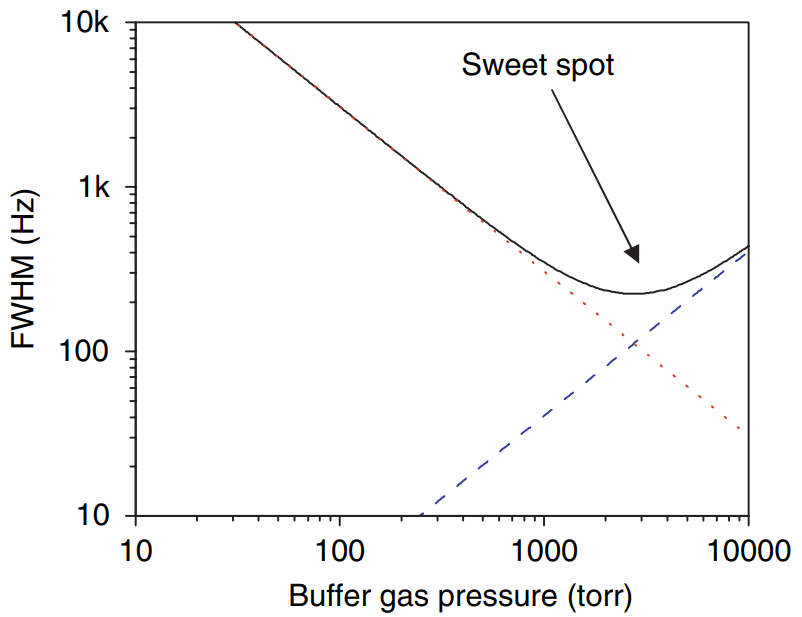
\includegraphics[width=0.7\textwidth]{img/extra-cell-pressure.png}
                \caption{Result of diffusion to the walls (red dotted line) and buffer gas collisions (dashed blue line).}
            \end{figure}

        \end{column}

        \begin{column}{0.5\textwidth}

            \begin{figure}
                \centering
                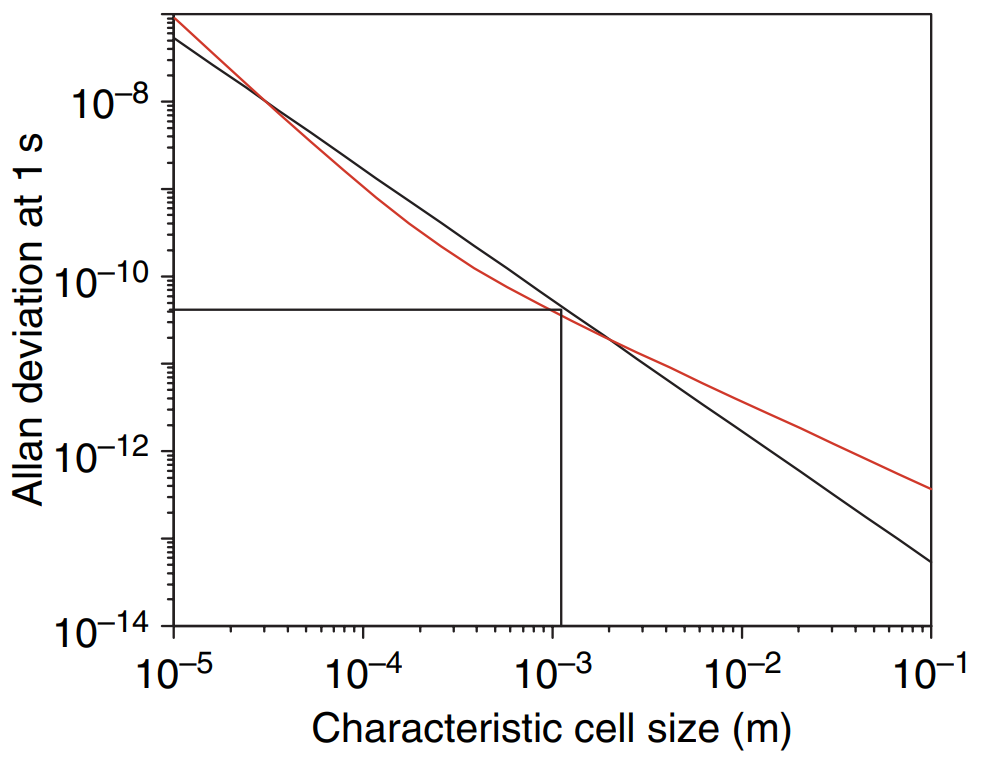
\includegraphics[width=0.7\textwidth]{img/extra-cell-size.png}
                \caption{Cell with a $100 kPa$ nitrogen buffer gas (red) or a paraffin wall coating (black).}
            \end{figure}

        \end{column}

    \end{columns}

    \footnotetext{FWHM: Full Width at Half Maximum}

\end{frame}



\begin{frame}{Quantum levels of $^{133}Cs$ and $^{87}Rb$}

    \begin{columns}[c, onlytextwidth]

        \begin{column}{0.5\textwidth}

            \begin{figure}
                \centering
                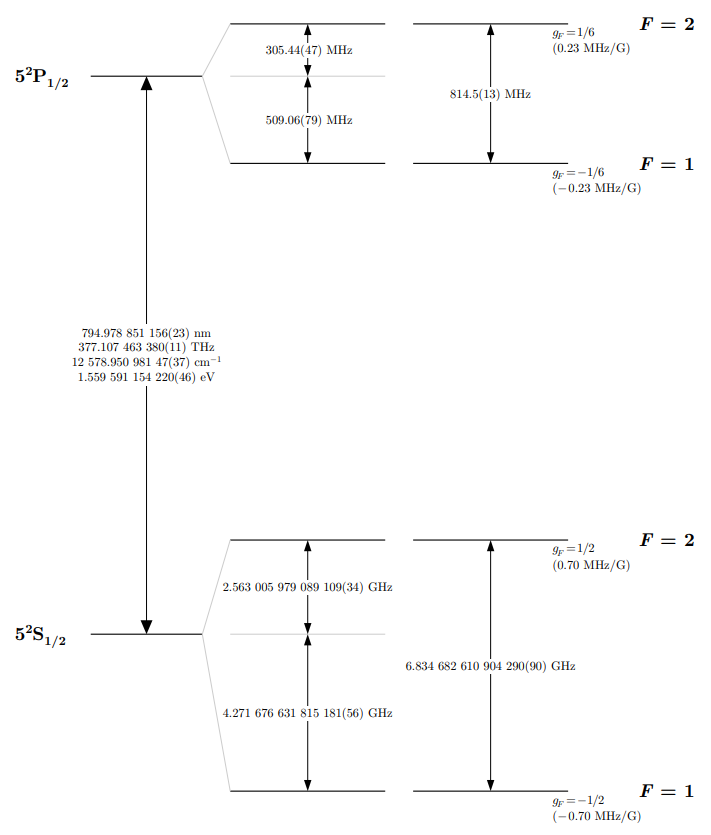
\includegraphics[height=0.7\textheight]{img/levels-Rubidium.png}
                \caption{$^{87}Rb$ quantum level.}
            \end{figure}

        \end{column}

        \begin{column}{0.5\textwidth}

            \begin{figure}
                \centering
                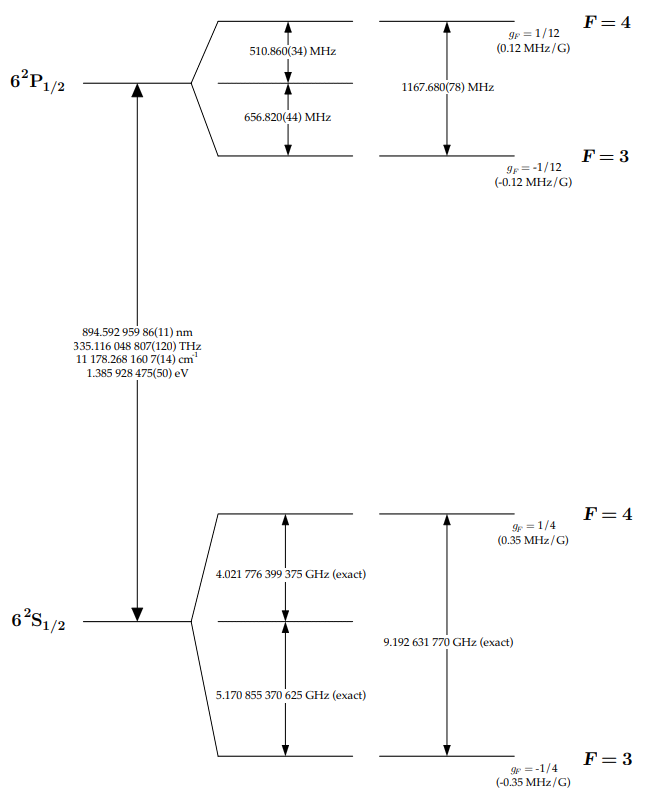
\includegraphics[height=0.7\textheight]{img/levels-Caesium.png}
                \caption{$^{133}Cs$ quantum level.}
            \end{figure}

        \end{column}

    \end{columns}

\end{frame}



\begin{frame}{Zeeman effect and c-field for clock calibration}

    The Zeeman effect is the splitting of atomic energy levels due to the presence of an external magnetic field.

    \begin{figure}
        \centering
        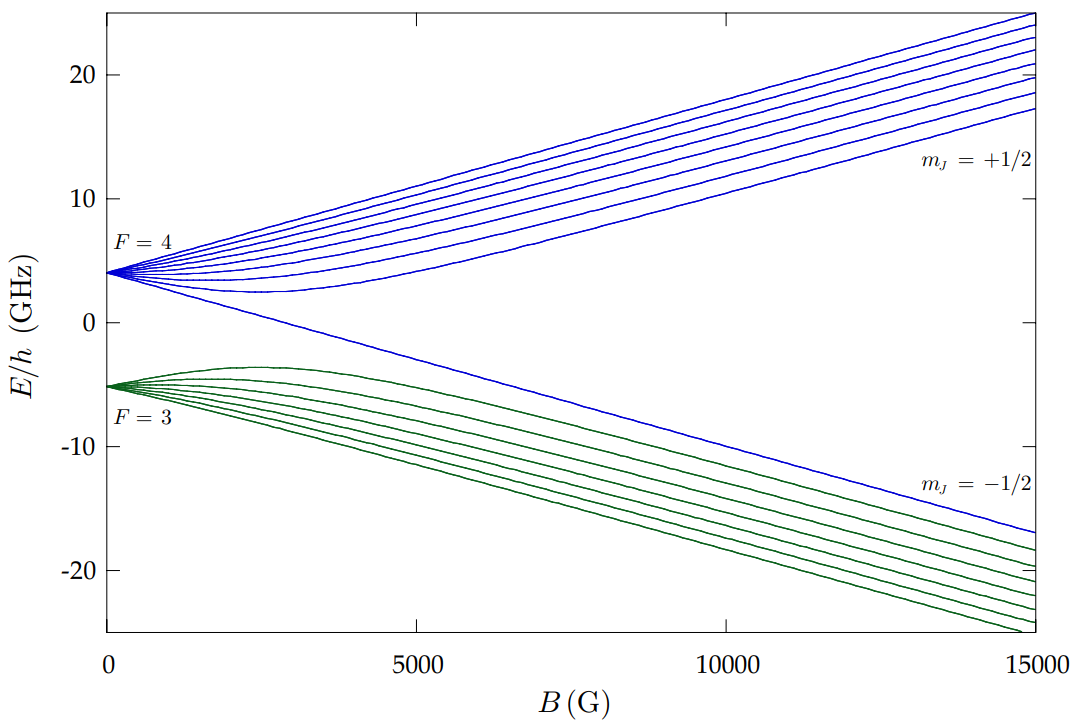
\includegraphics[width=0.5\textwidth]{img/extra-zeeman-splitting.png}
        \caption{$^{133}Cs$ $6S_{1/2}$ (ground) level hyperfine structure in an external magnetic field}
    \end{figure}

    A fine calibration of the clock can be done by applying a c-field (controlled magnetic field) to the reference cell.

\end{frame}
